\documentclass{article}

\usepackage{ctex}
\usepackage{graphicx}
\usepackage{float}
\usepackage{datetime}
\usepackage{hyperref}
\usepackage{amssymb}
\usepackage{amsthm}
\newtheorem{theorem}{Theorem}
\newtheorem{corollary}{Colollary}
\newtheorem{lemma}{Lemma}
\newtheorem{definition}{Definition}
\renewcommand\proofname{Proof}
\renewcommand\figurename{Figure}
\usepackage{listings}
\usepackage{xcolor}
\usepackage[linesnumbered, ruled]{algorithm2e}
\usepackage[legalpaper, margin=1.4in]{geometry}

\title{CS216 Assignment4 \\ {\begin{large} Description of the subtree disassembly trick proposed by Tarjan \end{large}}}  %title

\author{匡亮(12111012)}

\date{May 1, 2023}  % date

\begin{document}

\maketitle

\renewcommand\abstractname{Abstract}
\begin{abstract}

This is my report of CS216 Assignment4, including a description of the subtree disassembly trick proposed by Tarjan:

\begin{itemize}
    \item[1.] Its core idea and critical procedures.
    \item[2.] Running time and space complexity analysis.
    \item[3.] Its pseudocode.
    \item[4.] How it speeds up SPFA.
\end{itemize}

\end{abstract}

\newpage % contents page

\renewcommand\contentsname{Contents}
\tableofcontents

\newpage  % 1st page here

\section{Core idea and critical procedures of Tarjan's trick}

For convenience, in the whole report we assume the terminus vertex $t$ is reachable from every vertex in $G$, and our algorithm will immediately terminate if we find a negative ring (though some vertices cannot reach it, which means they still have a valid non-infinite minimum distance to the terminus vertex). Under these conditions, Tarjan's trick can significantly speed up SPFA without change the algorithm a lot.

Here I don't repeat what we have learned in our courses (like how SPFA works) and begin from SPFA.

In SPFA, we maintain an array $first$ for each vertex, and check whether there is a ring after $n$ iterations to determine whether there is a negative ring. However, if we have found a ring during the iterations, we can immediately terminate the algorithm and report there is a negative ring. Therefore, the basic idea of this trick is try to detect whether there is a ring when modifying $first$ with an acceptable extra cost.

Obviously, before we find a ring, $(v, first[v]),\forall v\not=t$ is a tree with root $t$. When we set $first[v]\leftarrow w$, we can do DFS in $v$'s subtree and check whether $w$ is in $v$'s subtree, if so, we can terminate our algorithm. However, this DFS will cost an extra $O(n)$ time, so we should expect it to do more for us. We can further observe that before the modification, the minimum distance of all vertices in $v$'s subtree (call them $x$) is evaluated based on the minimum distance of $v$, which has been just modified. Therefore, the minimum distance of all of them are out of date. We can set them \textbf{dormant}, then they will not be used to update others' minimum distance before their own minimum distance are updated. At the same time we can remove them from the tree (set $first[x]\leftarrow null$), so that they will not be set dormant by other ancestors again. They will add themselves back to the tree automatically when their minimum distance are updated (because they will update $first[x]$ at that time).

\section{Running time and space complexity analysis}

Based on SPFA, we just store one more tree with $O(1)$ space per vertex, so the space complexity is still $O(n)$.

Add/Remove a vertex to/from the tree can be easily done in $O(1)$ time with linked-list. Adding only happens when $first[v]$ are updated for some $v$, and removing happens no more than adding because vertices will not be removed twice, so the time complexity is still $O(nm)$.

\newpage

\section{Pseudocode}

\begin{algorithm}
    \KwData{G, t}
    $n=$ number of nodes in $G$\;
    $foundNegativeRing=$ False\;
    Array $M[V]$\;
    Initialize $M[t]=0$ and $M[v]=\infty$ for all other $v\in V$\;
    Initialize $first[t]=t$ and $first[v]=null$ for all other $v\in V$\;
    Initialize a tree with only root vertex $t$\;
    Set all vertices except $t$ dormant in the first iteration\;
    \For {$i=1,...,n-1$} {
        Set all vertices dormant in next iteration\;
        \For {$w\in V$ where $w$ is not dormant in this iteration} {
            \For {all edges $(v,w)$} {
                $M[v]=\min(M[v],c_{vw}+W[w])$\;
                \If {this change the value of $M[v]$} {
                    $first[v]=w$\;
                    \For {all vertex $x$ in $v$'s subtree} {
                        \If {$x$ is equal to $w$} {
                            $foundNegativeRing=$ True\;
                            End the algorithm\;
                        }
                        Set $x$ dormant in next iteration\;
                        Remove $x$ from the tree\;
                    }
                    Set $v$ not dormant in next iteration\;
                    Add $v$ to the tree as $w$'s child\;
                }
            }
        }
        \If {no value changed in this iteration} {
            End the algorithm\;
        }
        \tcc { If $foundNegativeRing$ is true, then users should ignore the returned $M,first$. }
    }
    \KwResult{$foundNegativeRing,M,first$}
    \caption{SPFA Improved by Tarjan's Trick}
\end{algorithm}

\section{How it speeds up SPFA}

If there is a negative ring, the algorithm will terminate in advance, so it is speeded up without a doubt.

Even if there is no negative rings, this trick can still speed SPFA up. \textbf{Figure 1.} below shows a classic example.

\begin{figure}[h]  % 'h' means insert here
    \centering
    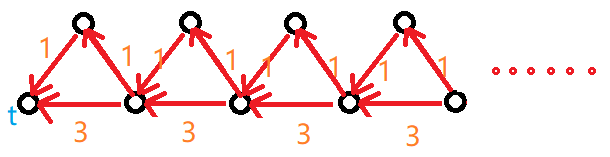
\includegraphics[height=2cm,width=8cm]{figure/1.png}
    \caption{An example forcing SPFA to run for $\Omega(nm)$ time.}
    \label{1}
\end{figure}

In this example, the terminus vertex is on the leftmost, and the orange numbers are weights. If we update all vertices from left to right, we will always first update the vertex on the lower left corner of a triangle, and then the vertex on the upper angle, which will update the vertex on the lower left corner in the next iteration. In short, the vertices on the lower layer have been always misleading in the whole procedure. Actually, in the $a$th round for $a<\frac{n}{2}$, there are $2a-1$ vertices being updated in the last iteration. However, if we use Tarjan's trick, there will always be $O(1)$ vertices need to be operated in each iteration. Thouth the misleading still exists, it will not bring extra cost to us because we can always immediately detect it and set the misled vertices dormant.

We can think in another way. Recall that SPFA calculates the minimum distance from $v$ to $t$ with no more than $i$ edges for all vertices $v$ in the $i$th iteration. In this example, the $i$th lower layer vertex from right has $i$ different minimum distances, each of them use different numbers of edges, so its value will be changed for $i$ times during the procedure. \textbf{Figure 2.} below shows an example for $i=3$. But if we use Tarjan's trick, we will keep focusing on minimizing the final answer and ignore those useless local answer.

\begin{figure}[h]  % 'h' means insert here
    \centering
    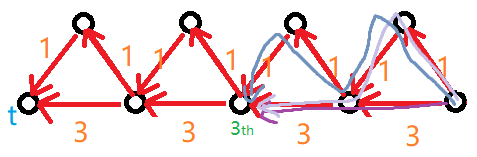
\includegraphics[height=2cm,width=8cm]{figure/2.png}
    \caption{An explanation for why SPFA runs slowly on this example.}
    \label{2}
\end{figure}

\newpage  % reference page

\renewcommand\refname{References}  % change '&' in the link to '\&'
\begin{thebibliography}{99}
    \bibitem[Jon Kleinberg / Éva Tardos(2005)]{textbook} Algorithm Design (P.304 - 307)

    \bibitem[Stefan Lewandowski(2010)]{article} Shortest Paths and Negative Cycle Detection in Graphs with Negative Weights - I: The Bellman-Ford-Moore Algorithm Revisited
    https://d-nb.info/1014960916/34

\end{thebibliography}

\end{document}
